\documentclass[aspectratio=169]{beamer}

\usepackage{amsmath,amssymb}
\usepackage{booktabs}
\usepackage{tabularx}
\usepackage{tikz}
\usetikzlibrary{arrows.meta,backgrounds,calc,positioning,shapes.multipart}
\usepackage[main=english]{babel}
\babelprovide[import]{polish}
\usepackage{ragged2e}
\usepackage{csquotes}
\usepackage{comment}
\usepackage[
  backend=biber,
  style=authoryear,
  maxcitenames=2,
  doi=false,
  isbn=false,
  url=true
]{biblatex}
\addbibresource{refs.bib}

\usetheme[
  accent=themeColorThree,
  progressbar=foot,
  sectionpage=progressbar,
  subsectionpage=none,
  numbering=fraction,
  numberrail=subsection,
  block=fill,
  notes=hide,
  toc=aftertitle,
  closing=contact
]{cookie}

\lstset{style=cookie}

\title[ISA4RL]{Instance Space Analysis for Reinforcement Learning}
\subtitle{Characterizing Algorithm Performance in Autonomous Driving Problems}
\author[F\'elix]{F\'elix Martins}
\thesissupervisor{Zafeiris Kokkinogenis}
\thesiscosupervisor{Daniel Castro Silva}
\thesisdegree{Masters in Artificial Intelligence}
\date{July 20, 2026}
\titlelogoone{
\includegraphics[width=.235\paperwidth]{figures/feup-logo.png}}
\titlelogotwo{
\includegraphics[width=.235\paperwidth]{figures/fcup-logo.png}}
\cookieclosingtitle{Thank you}
\cookieclosingtext{Questions, forks, and bug reports are welcome.}

\newsavebox{\cookieDemoPenguin}
\savebox{\cookieDemoPenguin}{\cookiepenguin[scale=.31]}
\newcommand{\cookiedemomathcomparisonbody}{%
  \footnotesize
  \setlength{\abovedisplayskip}{.24em}%
  \setlength{\belowdisplayskip}{.24em}%
  \begin{columns}[T,onlytextwidth]
    \column{.18\textwidth}
      \centering
      \cookiekicker{Lining}\par
      \vspace{.45em}
      1234567890

    \column{.18\textwidth}
      \centering
      \cookiekicker{Oldstyle}\par
      \vspace{.45em}
      \oldstylenums{1234567890}

    \column{.22\textwidth}
      \centering
      \cookiekicker{Accents}\par
      \vspace{.45em}
      $\hat{x},\;\check{x},\;\tilde{a},\;\bar{a},\;\dot{y},\;\ddot{y}$

    \column{.36\textwidth}
      \centering
      \cookiekicker{Differentials}\par
      \vspace{.45em}
      $\displaystyle \iiint f(x,y,z)\,\mathrm dx\,\mathrm dy\,\mathrm dz$
  \end{columns}

  \vspace{.30em}
  \begin{columns}[c,onlytextwidth]
    \column{.47\textwidth}
      \[
        \frac{1}{\displaystyle 1+
          \frac{1}{\displaystyle 2+
          \frac{1}{\displaystyle 3+x}}}
        +
        \frac{1}{1+\frac{1}{2+\frac{1}{3+x}}}
      \]

    \column{.47\textwidth}
      \[
        F:\left|\begin{array}{ccc}
          F''_{xx} & F''_{xy} & F'_x \\
          F''_{yx} & F''_{yy} & F'_y \\
          F'_x     & F'_y     & 0
        \end{array}\right|=0
      \]
  \end{columns}

  \vspace{.02em}
  \begin{columns}[c,onlytextwidth]
    \column{.30\textwidth}
      \[
        \mathop{\int\!\!\!\int}_{\mathbf{x}\in\mathbb R^2}
        \!\langle \mathbf{x},\mathbf{y}\rangle\,\mathrm d\mathbf{x}
      \]

    \column{.34\textwidth}
      \[
        \overline{\overline{a\alpha}^2+\underline{b\beta}
        +\overline{\overline{d\delta}}}
      \]

    \column{.30\textwidth}
      \[
        \left]0,1\right[+\lceil x\rfloor-\langle x,y\rangle
      \]
  \end{columns}

  \vspace{.05em}
  \begin{columns}[c,onlytextwidth]
    \column{.44\textwidth}
      \[
        \begin{aligned}
          e^x &\approx 1+x+x^2/2! \\
              &\quad{}+x^3/3!+x^4/4!
        \end{aligned}
      \]

    \column{.50\textwidth}
      \[
        \binom{n+1}{k}=\binom{n}{k}+\binom{n}{k-1}
      \]
  \end{columns}

  \vspace{-.15em}
  {\scriptsize
  \[
    \begin{aligned}
      p(R,\phi)
      &\sim \int_{-\infty}^{\infty}
      \frac{
        \tilde{W}_n(\gamma)
        \exp\!\left[
          \imath R/a
          \left(\sqrt{k^2a^2-\gamma^2}\cos\phi\right)
        \right]
      }{
        \left(k^2a^2-\gamma^2\right)^{3/4}
      }\\[-.15em]
      &\qquad{}\times
      \frac{1}{
        {H_n^{\prime}}_n^{(1)}
        \left(\sqrt{k^2a^2-\gamma^2}\right)
      }\,d\gamma .
    \end{aligned}
  \]
  }%
}
\begin{document}

\maketitle

\section{Context}

\subsection{Reinforcement Learning}
\begin{frame}{Reinforcement Learning}
  \begin{columns}[T,onlytextwidth]
    \column{0.55\textwidth}
    \centering
    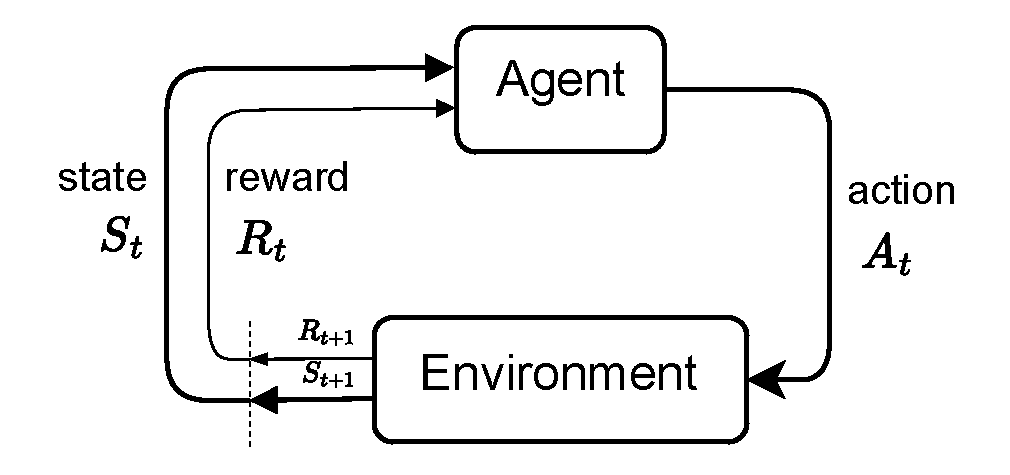
\includegraphics[width=\linewidth]{figures/basic-rl-diagram.pdf}
    \column{0.35\textwidth}
    \begin{itemize}
      \item Effective in complex decision problems
      \item No single algorithm outperforms others in all types of problems
      \item Requires heavy tuning and configuration
    \end{itemize}
  \end{columns}
\end{frame}

\subsection{Instance Space Analysis}
\begin{frame}{Instance Space Analysis (ISA)}
  \centering
  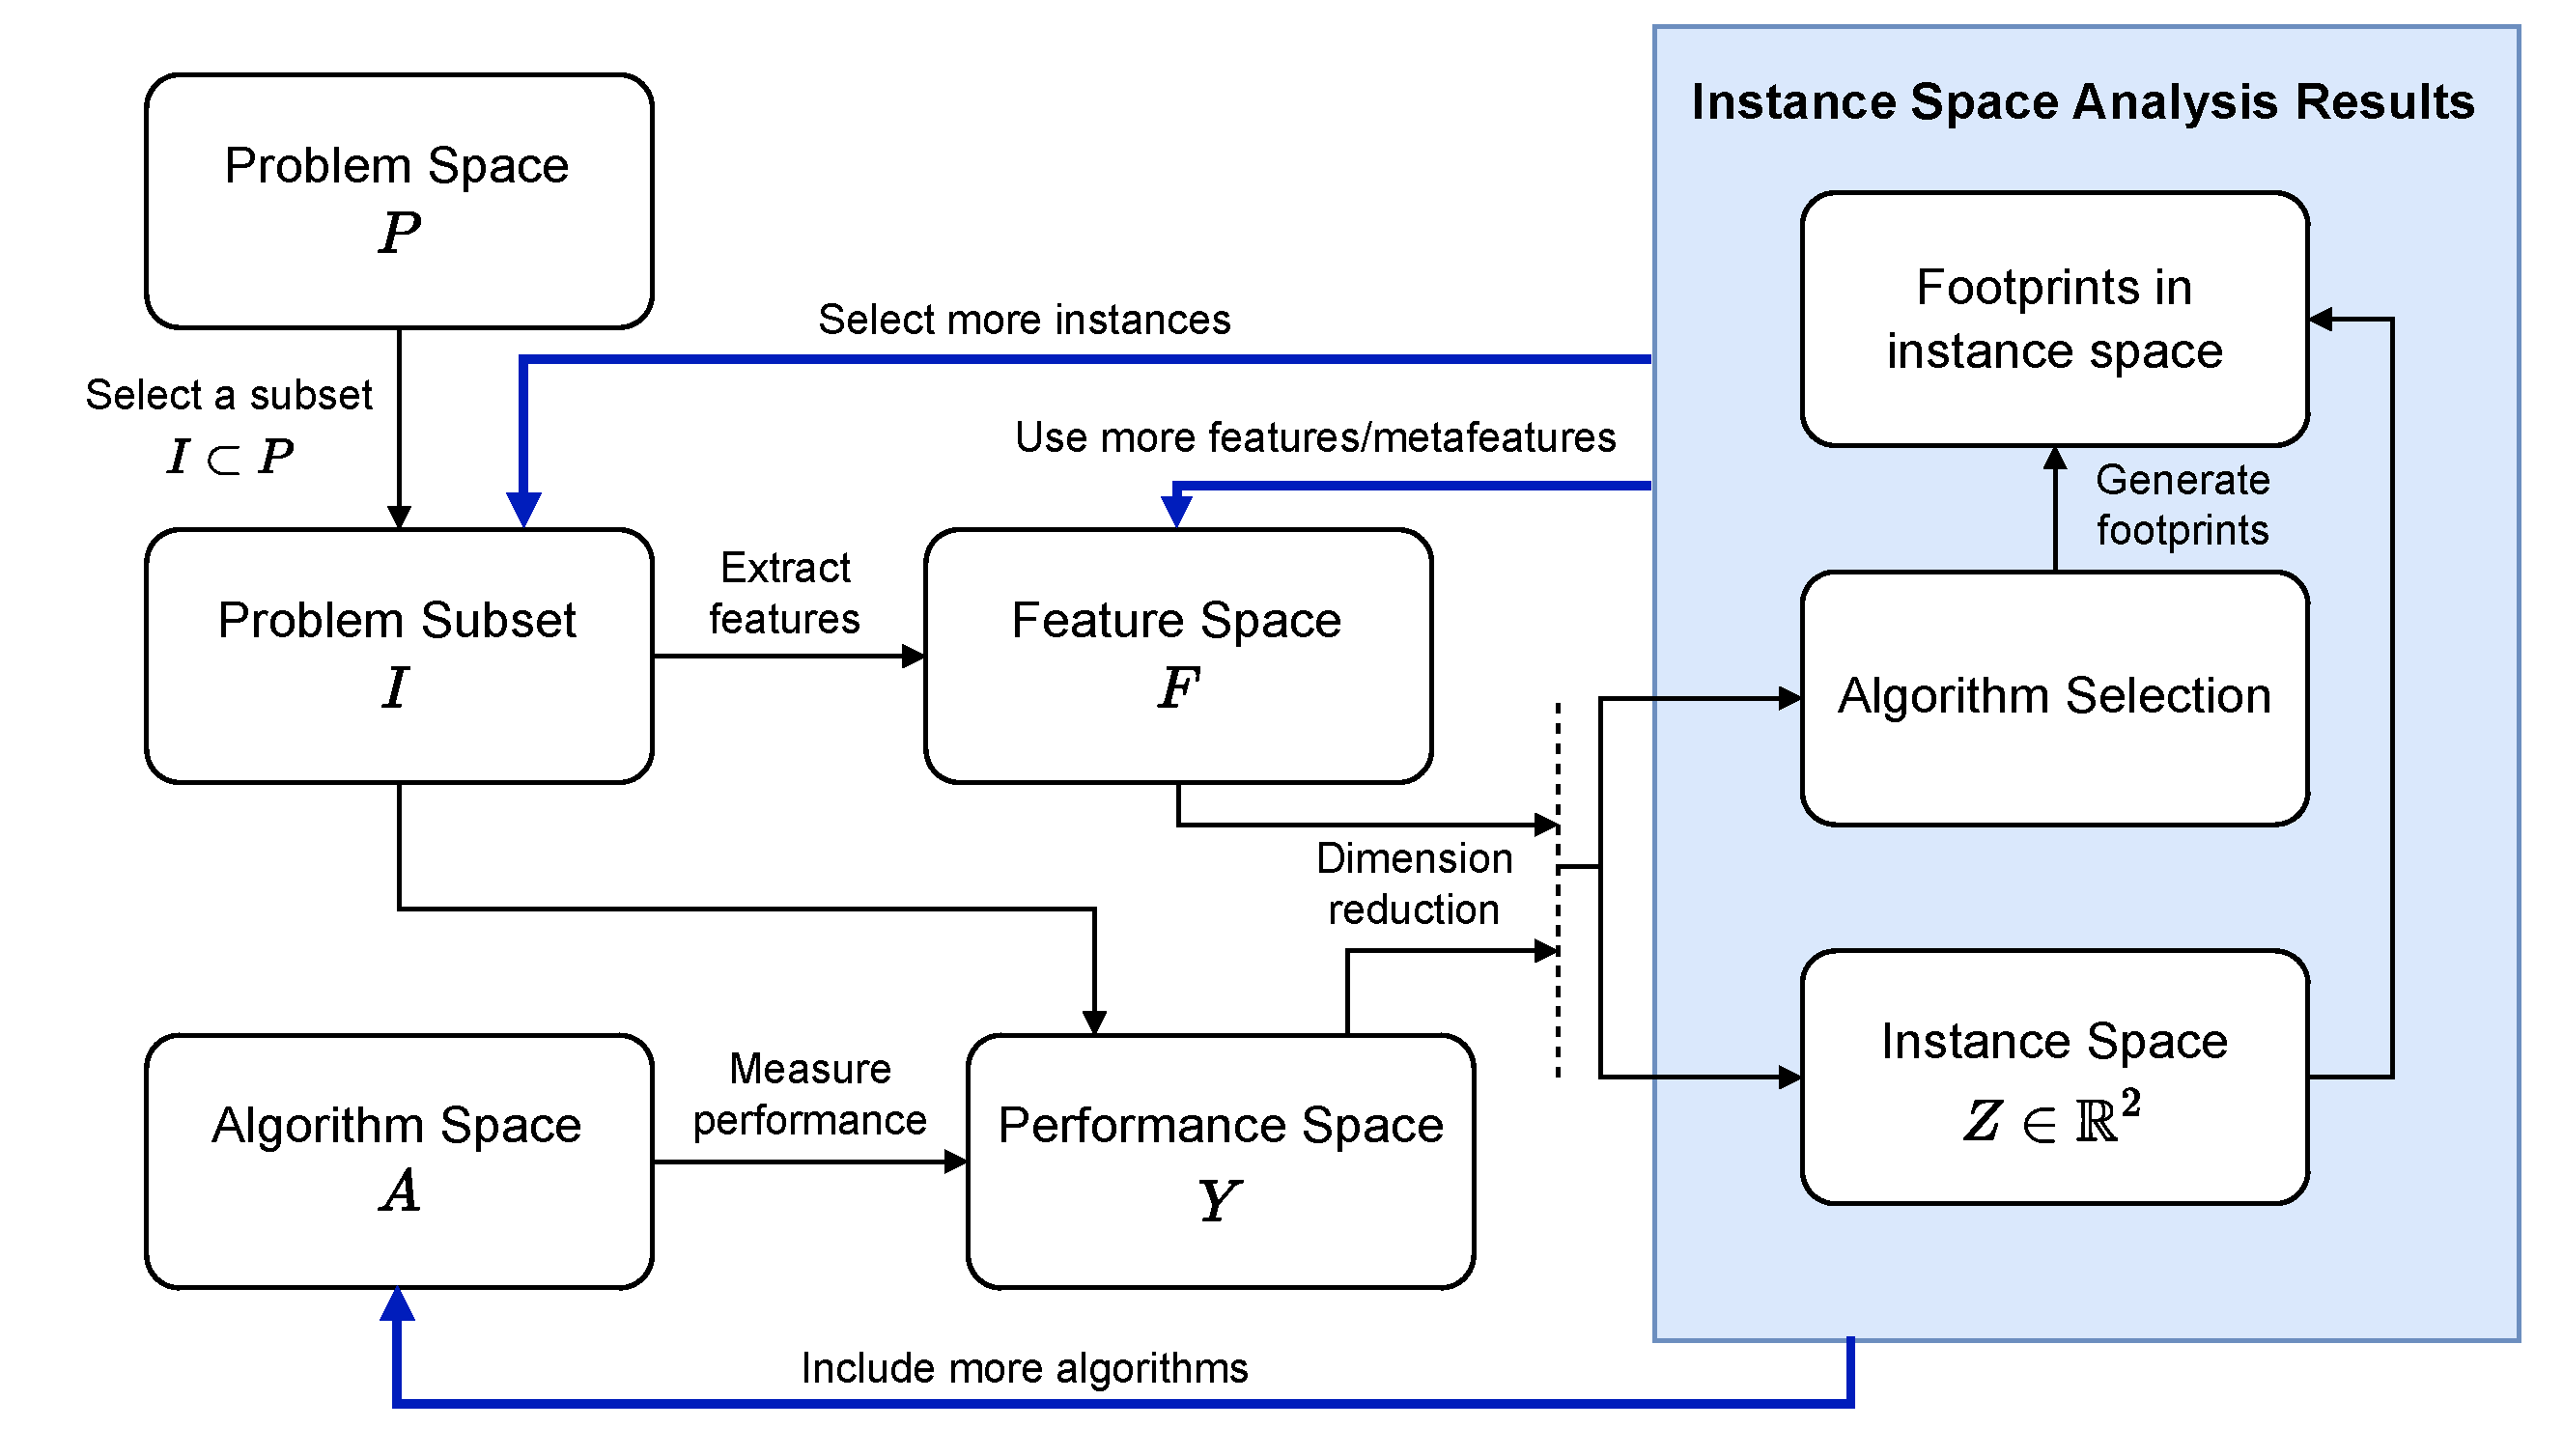
\includegraphics[width=0.75\linewidth]{figures/fw-isa.pdf}
\end{frame}

\begin{frame}{Instance Space Analysis: Example}
  \begin{columns}
    \column{0.6\textwidth}
    \centering
    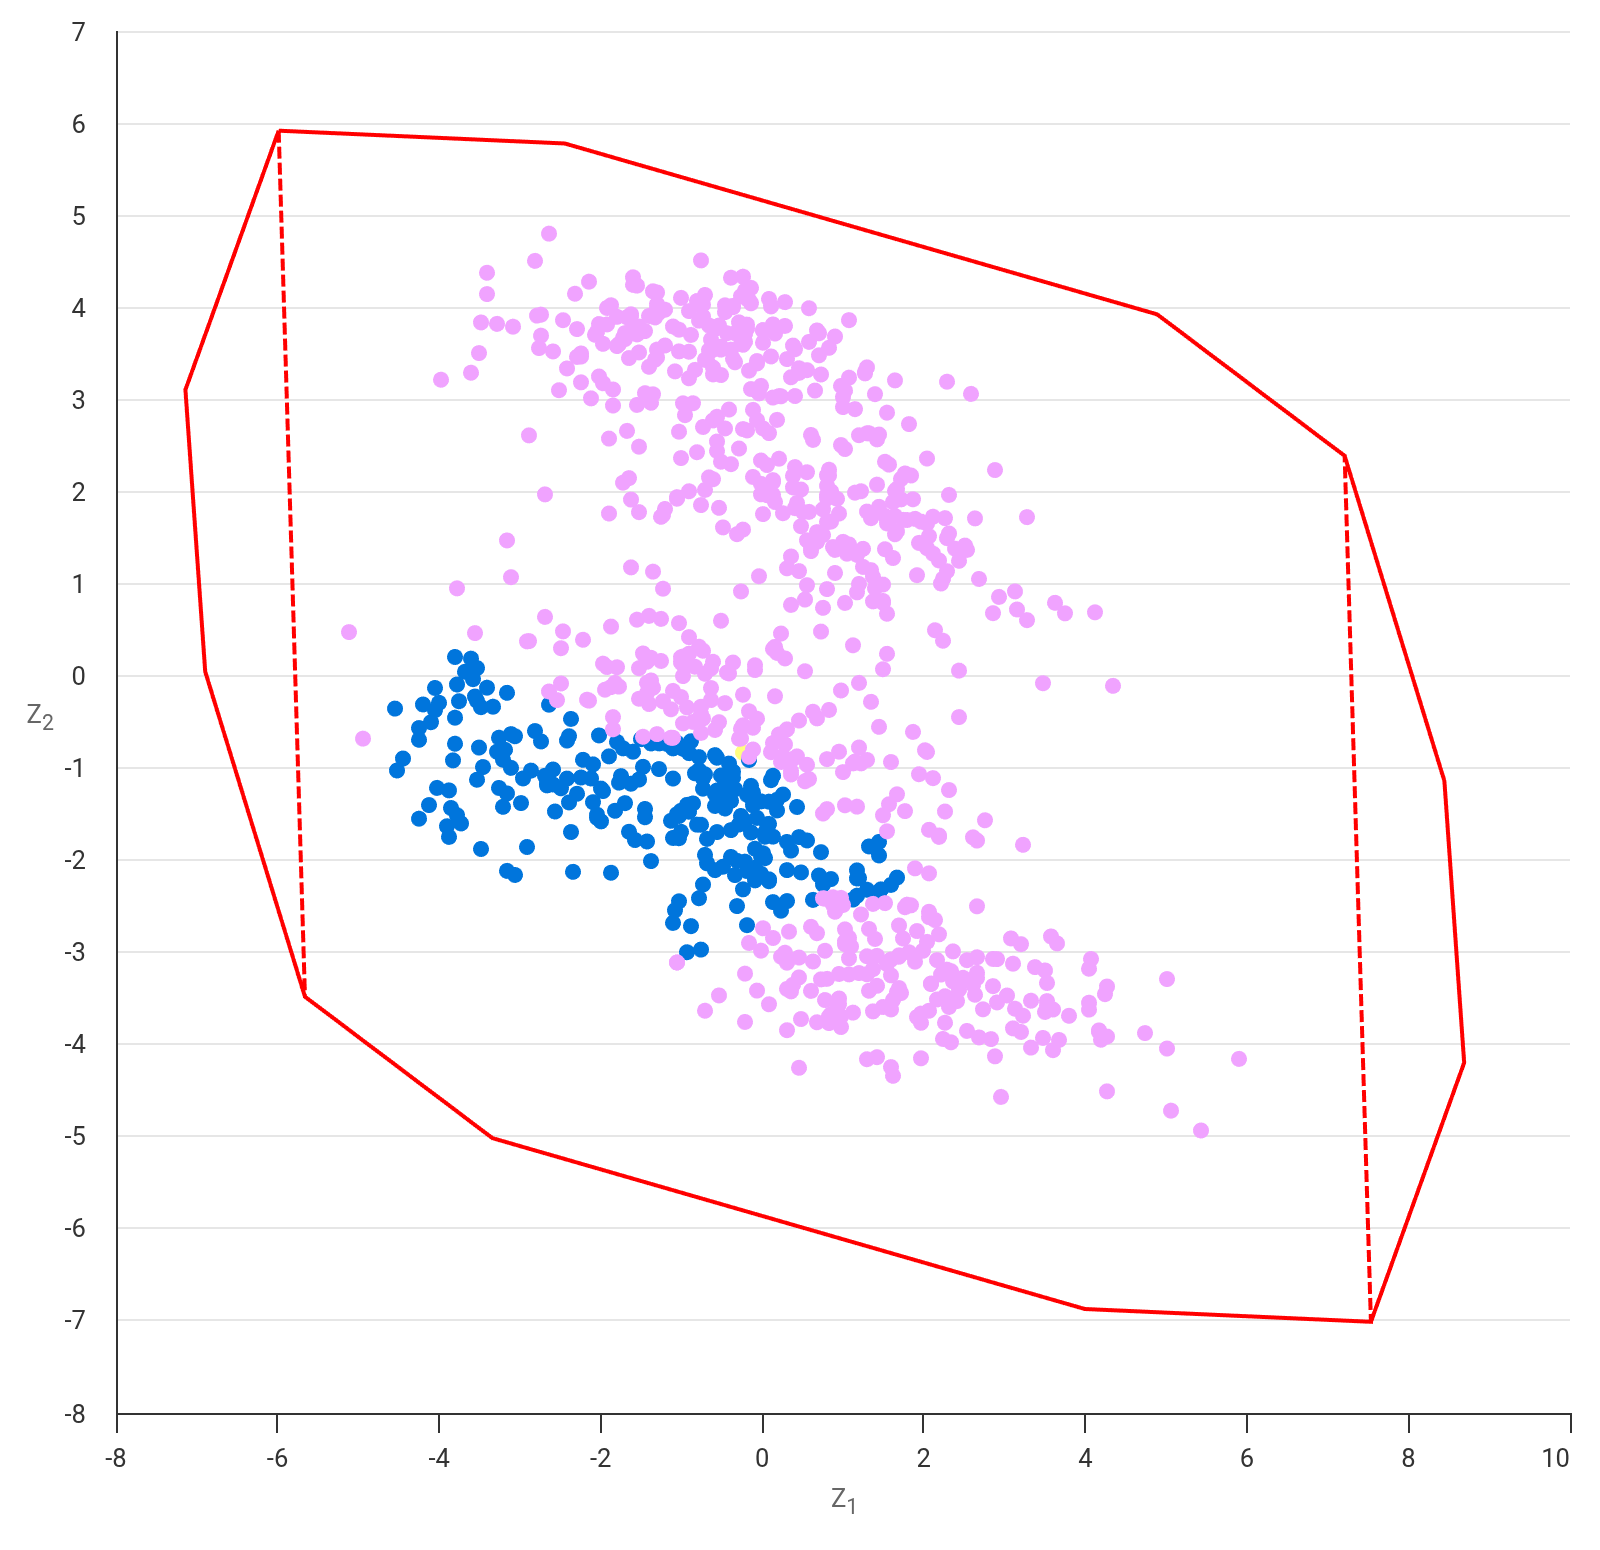
\includegraphics[width=0.7\linewidth]{figures/example_svm_selection.png}

    \vspace{0.25em}

    Example ISA algorithm selection for the Travelling Salesman %
    Problem~\cite{isa_discussing_suitability_tsp}.

    \column{0.3\textwidth}
    \scriptsize
    \begin{tabular}{@{}lc@{}}
      \toprule
      \textbf{Algorithms} & \textbf{Success Rate} \\
      \midrule
      CLK  & 0.2 \\
      LKCC & 0.8 \\
      \textbf{Selector} & \textbf{0.907} \\
      \bottomrule
    \end{tabular}
  \end{columns}
\end{frame}

\subsection{Metafeatures}
\begin{frame}{Metafeatures}
  High-level measurable characteristics that describe a task that can %
  be informative of algorithm performance. Should be:
  \begin{itemize}
    \item Highly discriminative
    \item Efficiently computable
    \item Independent of algorithms in study
  \end{itemize}
  
  Classication and regression have well-established metafeatures.

  ISA uses these metafeatures to capture the different properties of instances.

\end{frame}

\section{Literature Review}
\begin{frame}{Literature Review}
  A few issues arise to apply ISA to RL:
  \begin{itemize}
    \item No established metafeature set for RL
    \item Nonstationarity of RL: the actions of an agent affect the data it learns from;
    \item RL does not have a fixed dataset, only environment interactions;
  \end{itemize}

  Many works study properties that impact RL algorithm performance:
  \begin{itemize}
    \item Complexity Measures: capture the difficulty to solve a specific RL problem, %
    but are not efficiently computable for all problems
    \item Benchmarks: isolate environment properties and evaluate their impact on algorithms
  \end{itemize}

  Implicit knowledge of what impacts algorithm performance but no clear computable measures
\end{frame}

\section{Methodology}
\subsection{Simulators}
\begin{frame}{Simulators}{\ttfamily{HighwayEnv}}
  Minimalist environment designed for training simple RL agents for autonomous driving %
  decision-making.

  \vspace{.45em}
  \centering
  \begingroup
  \begin{minipage}[t]{.235\textwidth}
    \vspace{0pt}
    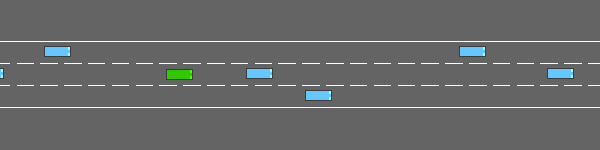
\includegraphics[width=\linewidth]{figures/sims/he/highway.png}
  \end{minipage}\hfill
  \begin{minipage}[t]{.235\textwidth}
    \vspace{0pt}
    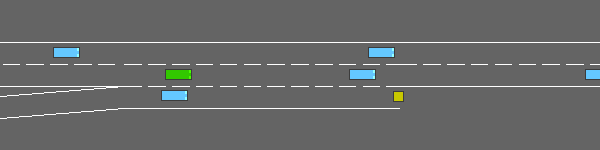
\includegraphics[width=\linewidth]{figures/sims/he/merge_image.png}
  \end{minipage}\hfill
  \begin{minipage}[t]{.235\textwidth}
    \vspace{0pt}
    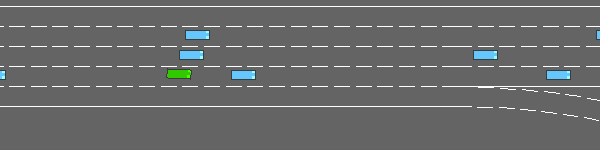
\includegraphics[width=\linewidth]{figures/sims/he/exit_image.png}
  \end{minipage}\hfill
  \begin{minipage}[t]{.235\textwidth}
    \vspace{0pt}
    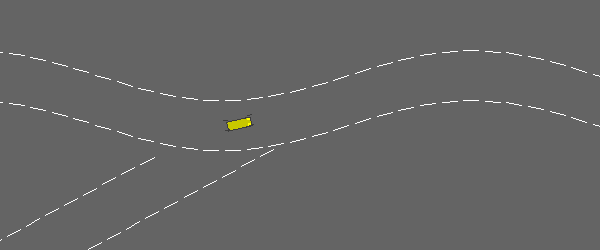
\includegraphics[width=\linewidth]{figures/sims/he/lane_keeping_smaller.png}
  \end{minipage}

  \vspace{.55em}
  \begin{minipage}[t]{.235\textwidth}
    \vspace{0pt}
    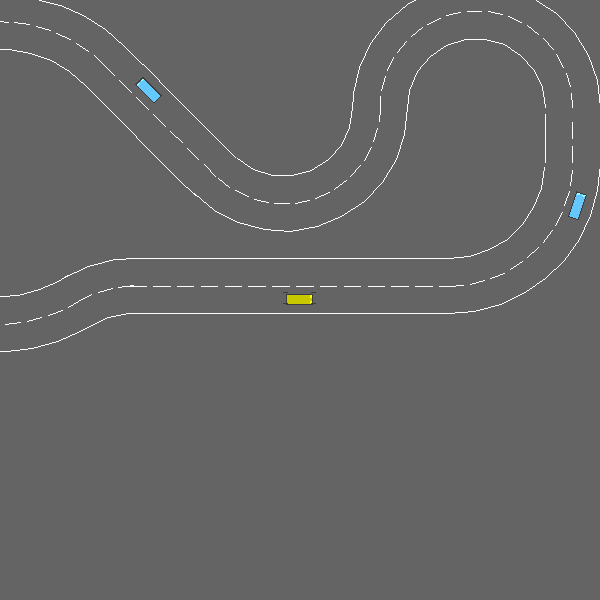
\includegraphics[width=\linewidth]{figures/sims/he/fixed_racetrack.png}
  \end{minipage}\hfill
  \begin{minipage}[t]{.235\textwidth}
    \vspace{0pt}
    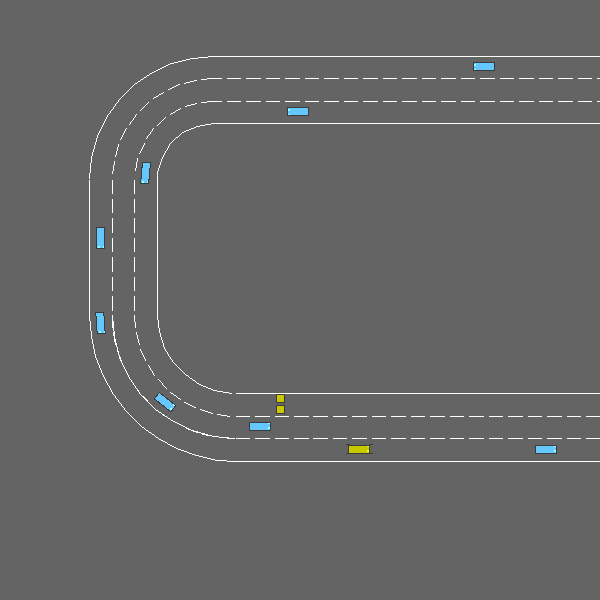
\includegraphics[width=\linewidth]{figures/sims/he/oval_racetrack.png}
  \end{minipage}\hfill
  \begin{minipage}[t]{.235\textwidth}
    \vspace{0pt}
    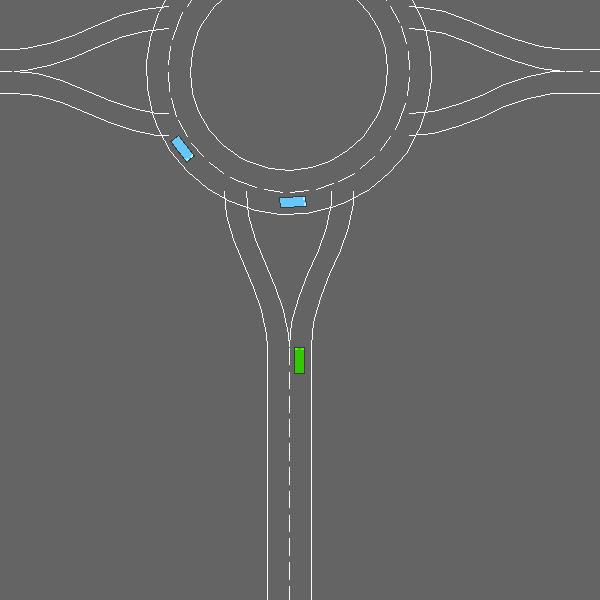
\includegraphics[width=\linewidth]{figures/sims/he/roundabout.png}
  \end{minipage}\hfill
  \begin{minipage}[t]{.235\textwidth}
    \vspace{0pt}
    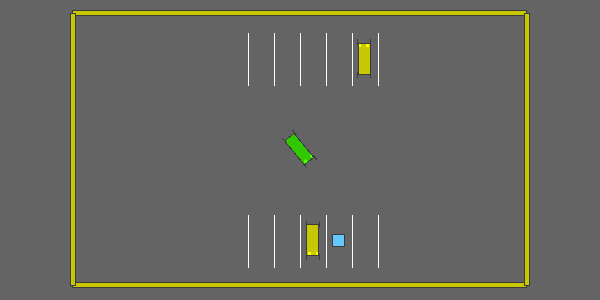
\includegraphics[width=\linewidth]{figures/sims/he/parking.png}
  \end{minipage}
  \endgroup
\end{frame}

\begin{frame}{Simulators}{MetaDrive}
  Designed to efficiently train generalizable RL agents using procedurally generated of maps.

  \vspace{.45em}
  \centering
  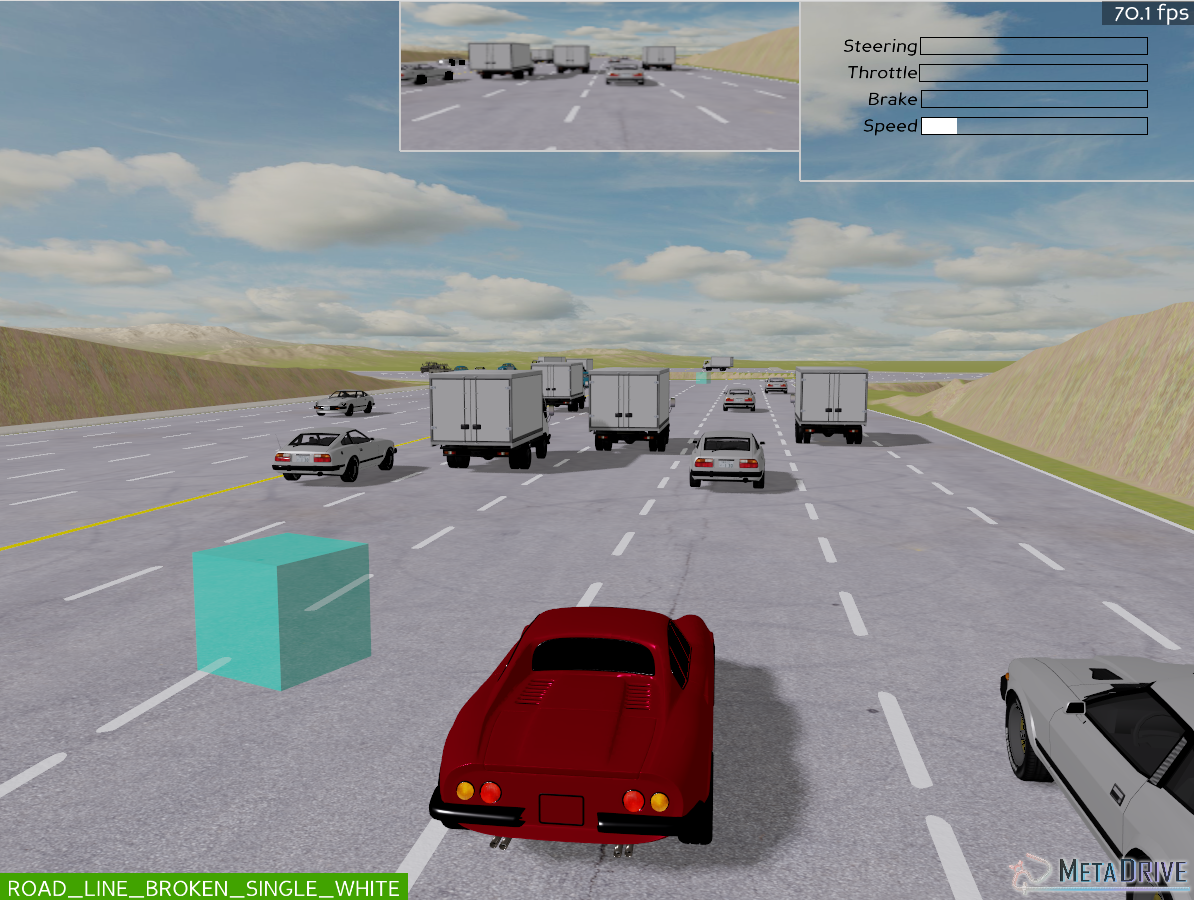
\includegraphics[width=0.5\linewidth]{figures/sims/md/md.png}
\end{frame}

\begin{frame}{Simulators}{MetaDrive Maps}
  \centering
  \begingroup
  \begin{minipage}[t]{.29\textwidth}
    \vspace{0pt}
    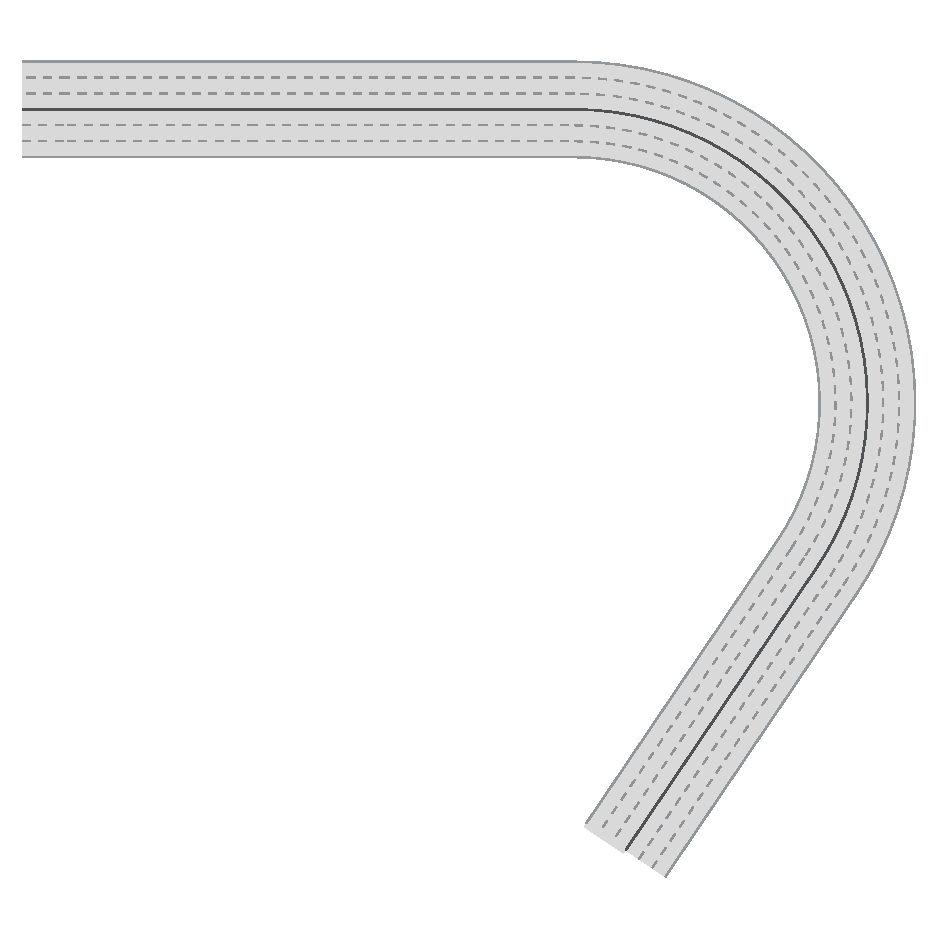
\includegraphics[width=\linewidth]{figures/sims/md/maps/image_SC_vector.pdf}
  \end{minipage}\hfill
  \begin{minipage}[t]{.29\textwidth}
    \vspace{0pt}
    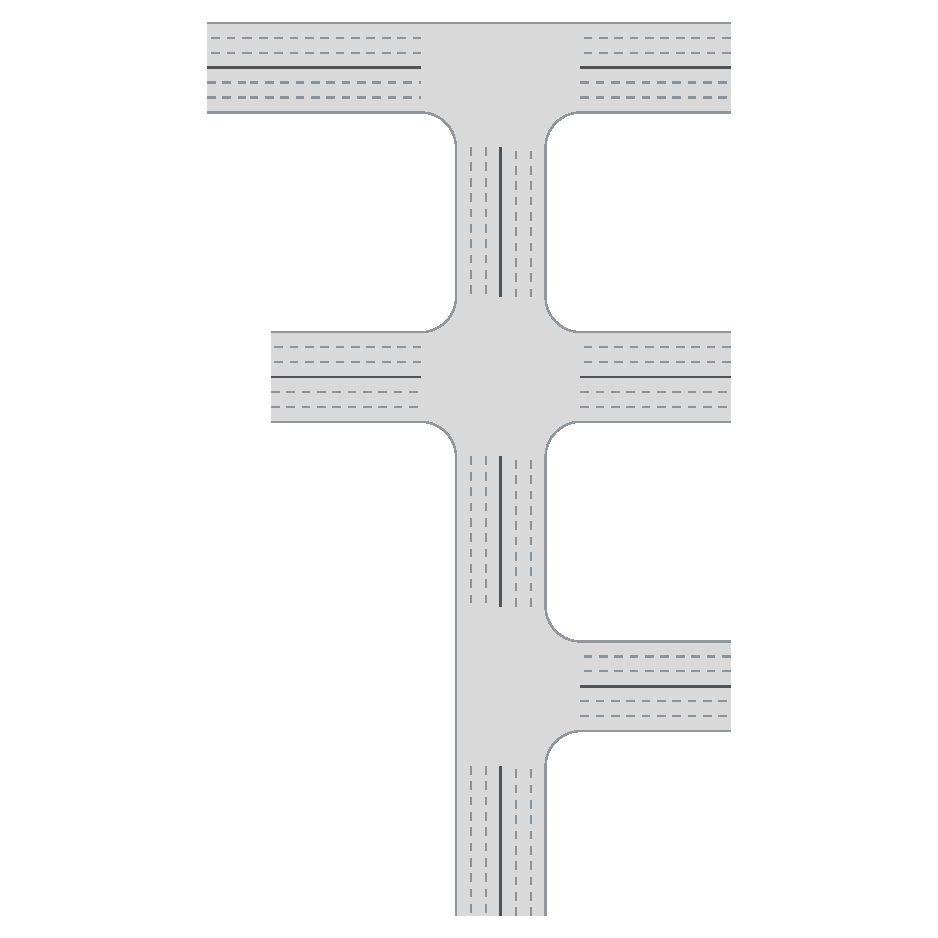
\includegraphics[width=\linewidth]{figures/sims/md/maps/image_TXT_vector.pdf}
  \end{minipage}\hfill
  \begin{minipage}[t]{.29\textwidth}
    \vspace{0pt}
    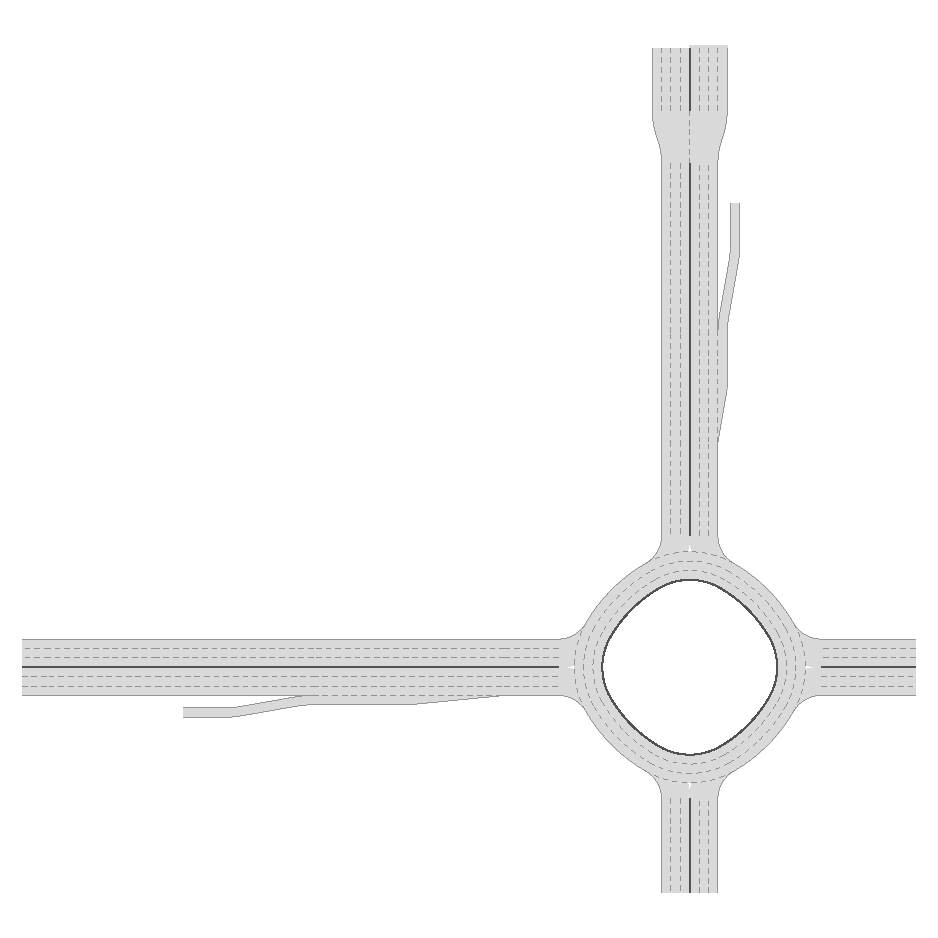
\includegraphics[width=\linewidth]{figures/sims/md/maps/image_rORY_vector.pdf}
  \end{minipage}
  \endgroup
\end{frame}

\begin{frame}{Simulators}{CARLA}
  High-fidelity simulator designed to evaluate state-of-the-art autonomous driving solutions.

  \vspace{.45em}
  \centering
  \begingroup

  \begin{minipage}[t]{.3\textwidth}
    \vspace{0pt}
    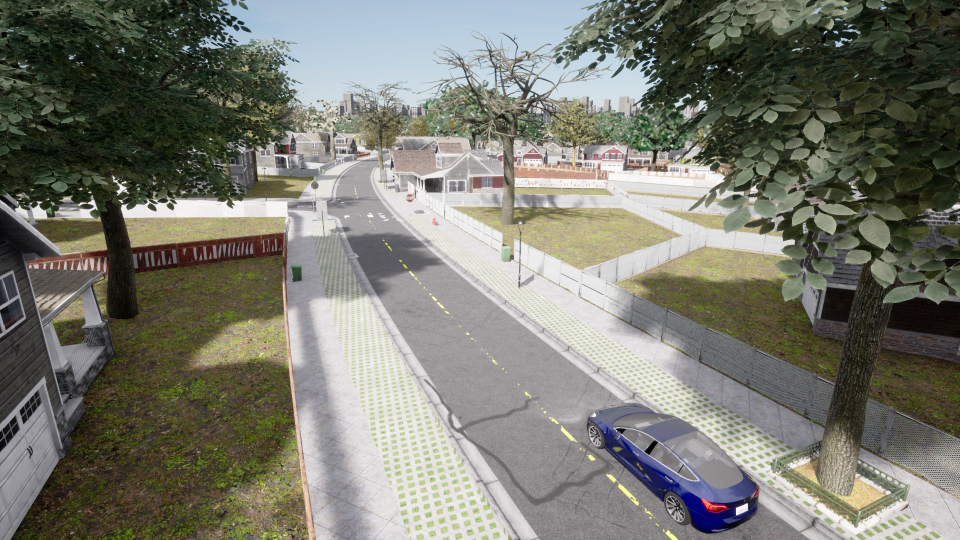
\includegraphics[width=\linewidth]{figures/sims/carla/road_and_intersection.png}
  \end{minipage}\hfill
  \begin{minipage}[t]{.3\textwidth}
    \vspace{0pt}
    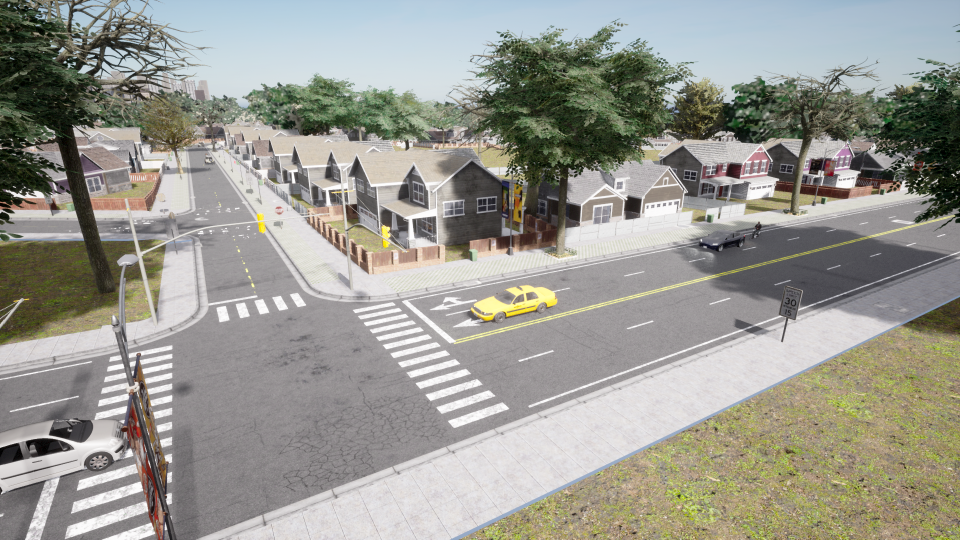
\includegraphics[width=\linewidth]{figures/sims/carla/intersection.png}
  \end{minipage}

  \vspace{.35em}
  \begin{minipage}[t]{.3\textwidth}
    \vspace{0pt}
    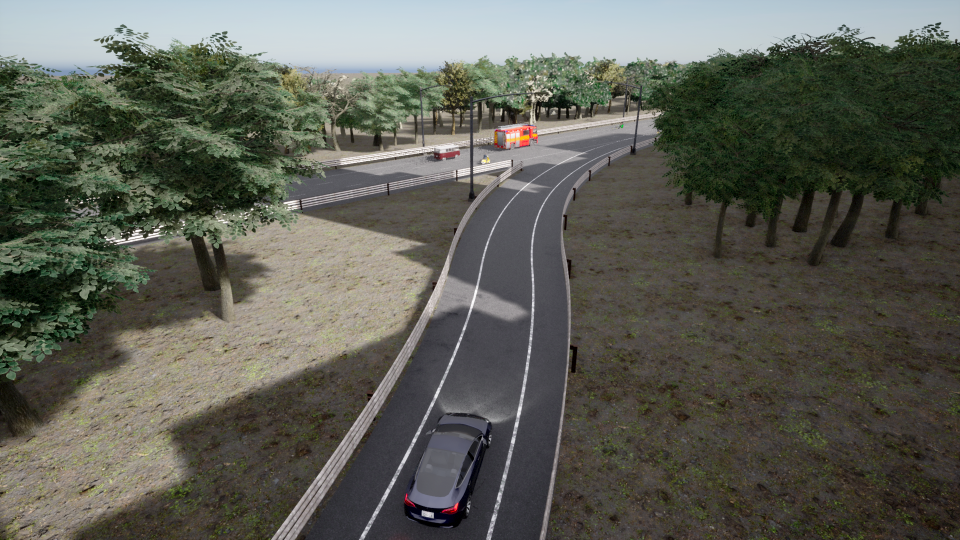
\includegraphics[width=\linewidth]{figures/sims/carla/highway_enter.png}
  \end{minipage}\hfill
  \begin{minipage}[t]{.3\textwidth}
    \vspace{0pt}
    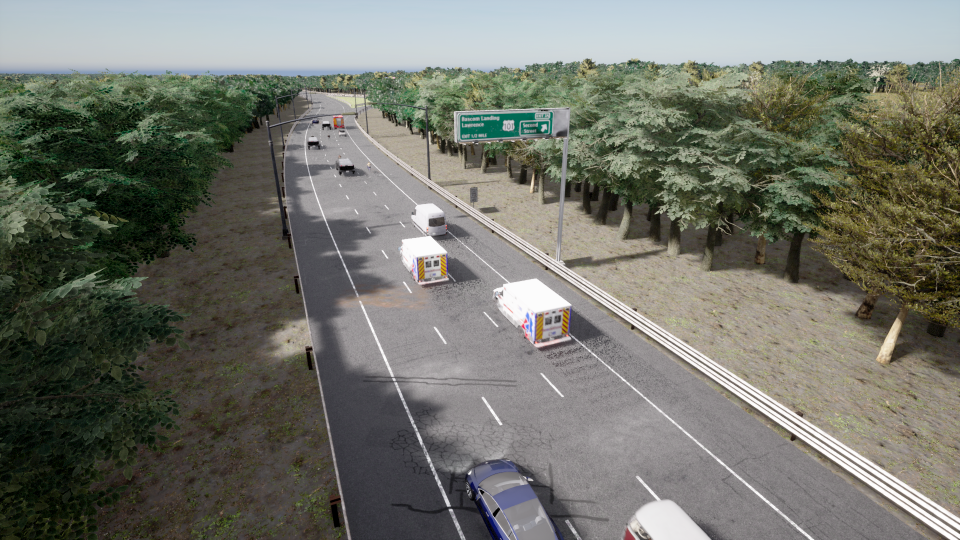
\includegraphics[width=\linewidth]{figures/sims/carla/highway_exit.png}
  \end{minipage}
  \endgroup
\end{frame}

\subsection{Pipeline}

\begin{frame}{Pipeline}
  \centering
  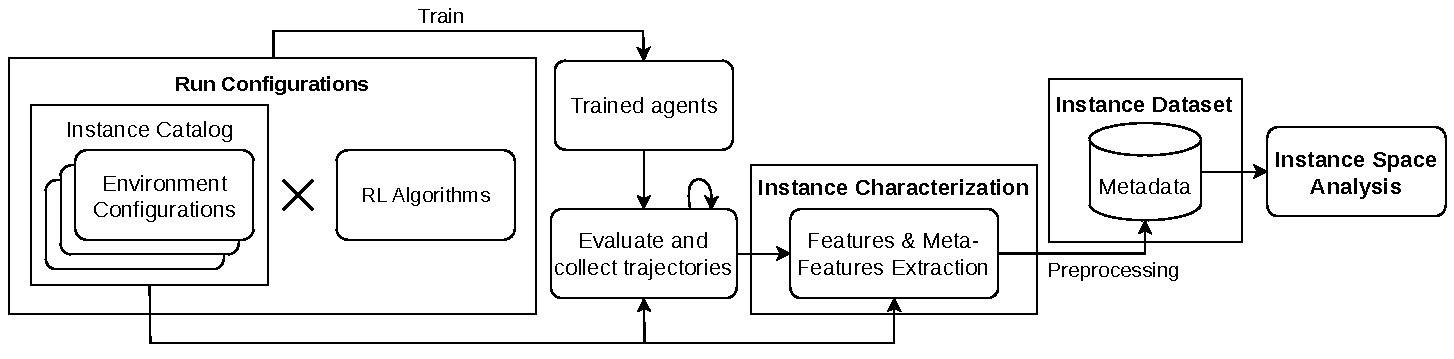
\includegraphics[width=\linewidth]{figures/meth_summary.pdf}
\end{frame}

\subsection{Instance Generation}

\begin{frame}{Instance Generation}
  To generate instances based on the chosen simulators, we vary several parameters %
  beyond the task or maps:
  \begin{itemize}
    \item Number of lanes
    \item Vehicle density and number of vehicles
    \item Other parameters such as road length, number of parking spots, \dots
  \end{itemize}
  This yields a total of 1073 instances: 845 for HighwayEnv, 210 for MetaDrive, and 18 for %
  CARLA, due to its much heavier and longer training and evaluation times.
\end{frame}

\subsection{RL Algorithms}

\begin{frame}{RL Algorithms}
  Algorithms and training/evaluation protocol from stable-baselines3~\cite{stable_baselines3}.

  RL algorithms may support discrete (D) and/or continuous (C) action spaces.
  \begin{itemize}
    \item \textbf{A2C}: D/C
    \item \textbf{DQN}: D
    \item \textbf{PPO}: D/C
    \item \textbf{SAC}: C
  \end{itemize}
  Fixed hyperparameter configuration for each instance, adapted based on observation space, %
  action space, and maximum episode timesteps
\end{frame}

\subsection{Metafeature Design}

\begin{frame}{Metafeature Design}
The main objective is to capture relevant aspects of each task.

To extract a dataset of trajectories, we use two simple non-learned %
``probe'' policies:
\begin{itemize}
  \item a random actions policy
  \item a rule-based heuristic baseline which depends on the environment
\end{itemize}

We define the following groups of metafeatures:
\begin{itemize}
  \item Environment structure
  \item Probe-performance and ego-dynamics
  \item Probe observation-stream
  \item Surrounding-traffic behavior
  \item Environment dynamics
\end{itemize}
\end{frame}

\subsection{Metadata Dataset}

\begin{frame}{Performance Normalization}
There is no general performance metric capable of comparing agent performance %
across heterogeneous environments.

\begin{itemize}
  \item An environment that yields higher mean returns may actually be harder to solve.
\end{itemize}

\vspace{0.45em}
To define performance, we use the random and baseline heuristic policies defined for %
the metafeature computation:
\[
s_{i,a} = \frac{R_{i,a} - R_{i,random}}{R_{i,baseline}-R_{i,random}}
\]
\begin{itemize}
  \item $s_{i,a}$: normalized performance metric for algorithm $a$
  \item $R_{i,a}$, $R_{i,random}$, $R_{i,baseline}$: mean episodic returns for the algorithm $a$, %
the random policy and the baseline heuristic policy, respectively.
\end{itemize}
\end{frame}

\section{Results}
\begin{frame}{Generating Instance Spaces}
  The ISA methodology requires defining specific hyperparameters by experimenting and iterating.
  We defined the most important parameters:
  \begin{itemize}
    \item Performance threshold for success: within 5\% of best-performing algorithm
    \item Number of selected features: 6 for discrete-action and 8 for continuous-action environments
  \end{itemize}

  % Analyzing individual environments provides context for multi-environment projections.
  % Results based on multiple environments provide more generalizable results.
\end{frame}

\subsection{Individual Environments}
\begin{frame}{Individual Environments}{\ttfamily{HighwayEnv} Highway projection}
  Resulting projection from selected features and dimension reduction:
  \vspace{0.4em}

  \centering
  \small
  \resizebox{.78\linewidth}{!}{$
    \begin{bmatrix}
      Z_1\\
      Z_2
    \end{bmatrix}
    =
    \begin{bmatrix}
      0.14 & -0.12 \\
      -0.50 & 0.32 \\
      0.35 & -0.41 \\
      0.50 & 0.37 \\
      0.09 & 0.38 \\
      -0.38 & -0.37 \\
      \end{bmatrix}^{T}
      \begin{bmatrix}
      \text{\tiny\ttfamily lanes-count} \\
      \text{\tiny\ttfamily traffic-density} \\
      \text{\tiny\ttfamily baseline-speed-snr} \\
      \text{\tiny\ttfamily baseline-obs-volatility-mean} \\
      \text{\tiny\ttfamily state-entropy} \\
      \text{\tiny\ttfamily action-state-discontinuity-p95}
    \end{bmatrix}
  $}
\end{frame}

\begin{frame}{Individual Environments}{Highway Sources and Best Algorithms}
  \begin{columns}[c,onlytextwidth]
    \column{.49\textwidth}
      \centering
      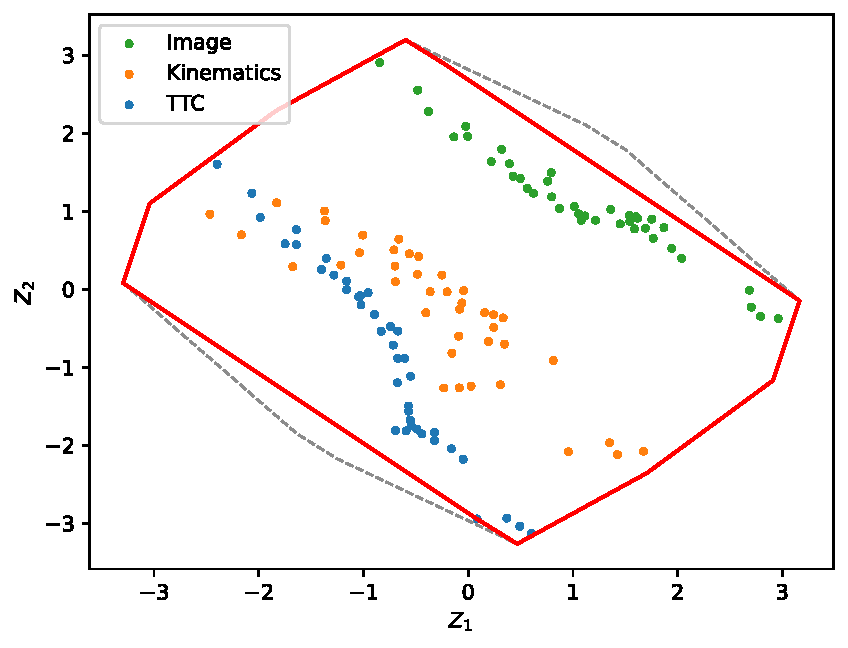
\includegraphics[width=\linewidth]{figures/results/single-envs/highway/7_sources.pdf}
      {Observation Space Type}

    \column{.49\textwidth}
      \centering
      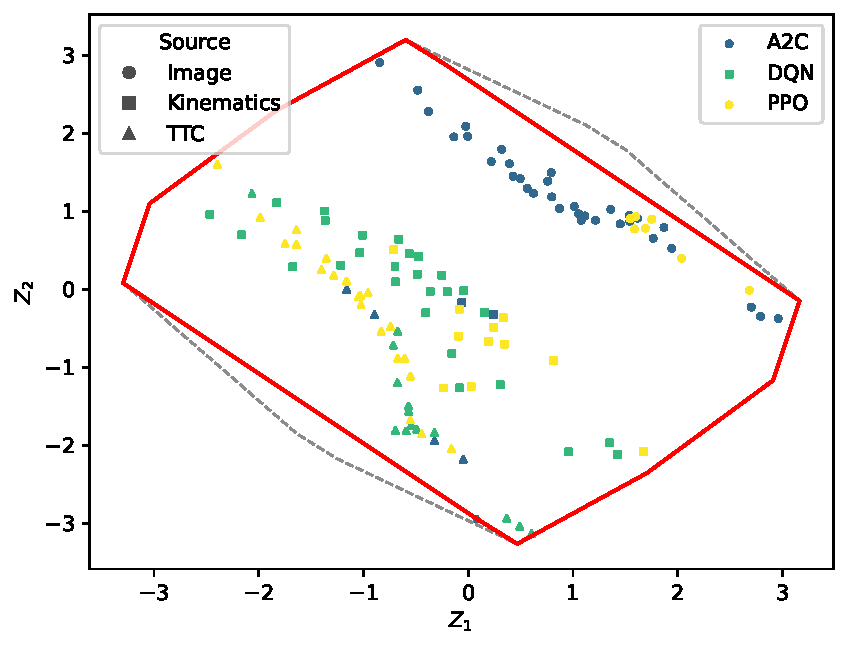
\includegraphics[width=\linewidth]{figures/results/single-envs/highway/5_port.pdf}
      {Best-Performing Algorithm}
  \end{columns}
\end{frame}

\begin{frame}{Individual Environments}{Highway Features Distribution}
  \centering
  \begingroup
  \setlength{\tabcolsep}{.25em}
  \begin{tabular}{ccc}
    \begin{minipage}[t]{.29\textwidth}
      \centering
      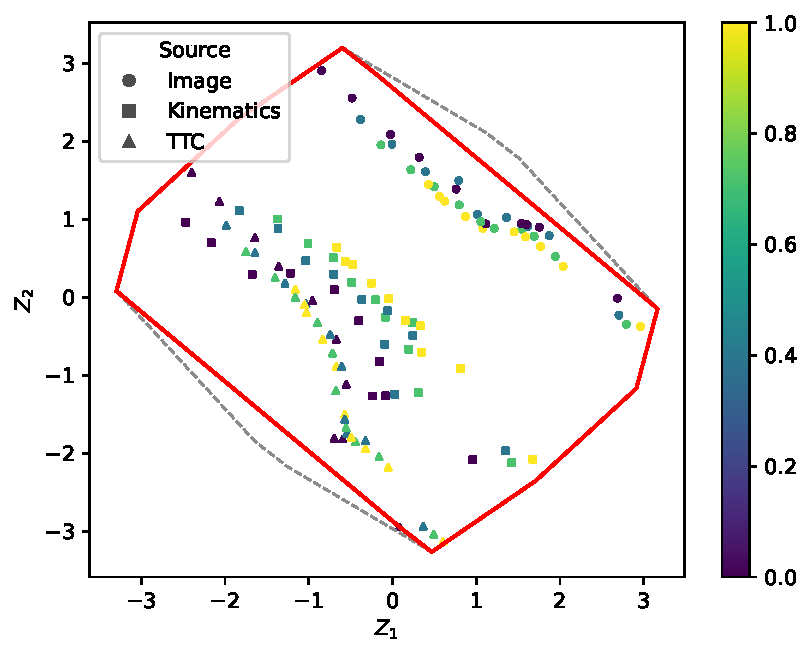
\includegraphics[width=.91\linewidth]{figures/results/single-envs/highway/2_lanes_count.pdf}
      {\tiny\ttfamily lanes-count\par}
    \end{minipage} &
    \begin{minipage}[t]{.29\textwidth}
      \centering
      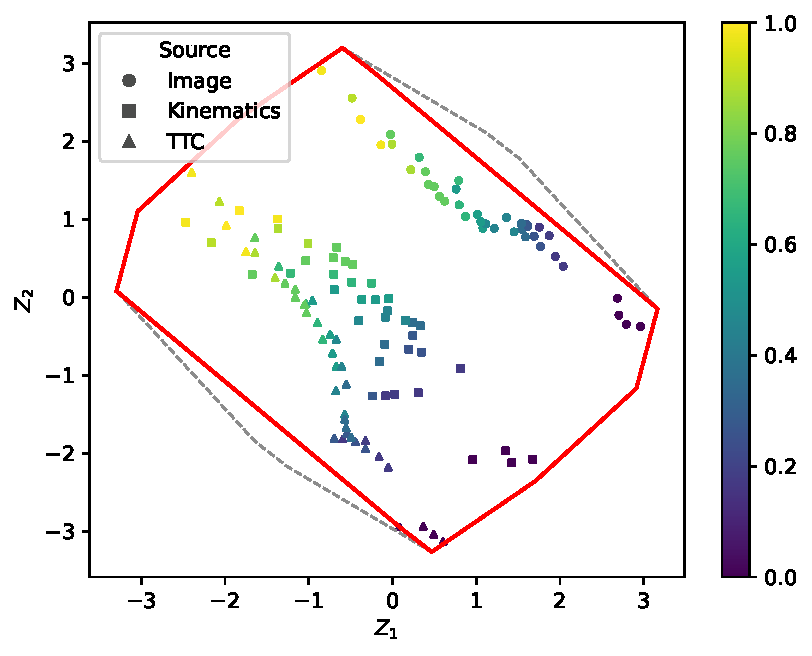
\includegraphics[width=.91\linewidth]{figures/results/single-envs/highway/2_traffic_density.pdf}
      {\tiny\ttfamily traffic-density\par}
    \end{minipage} &
    \begin{minipage}[t]{.29\textwidth}
      \centering
      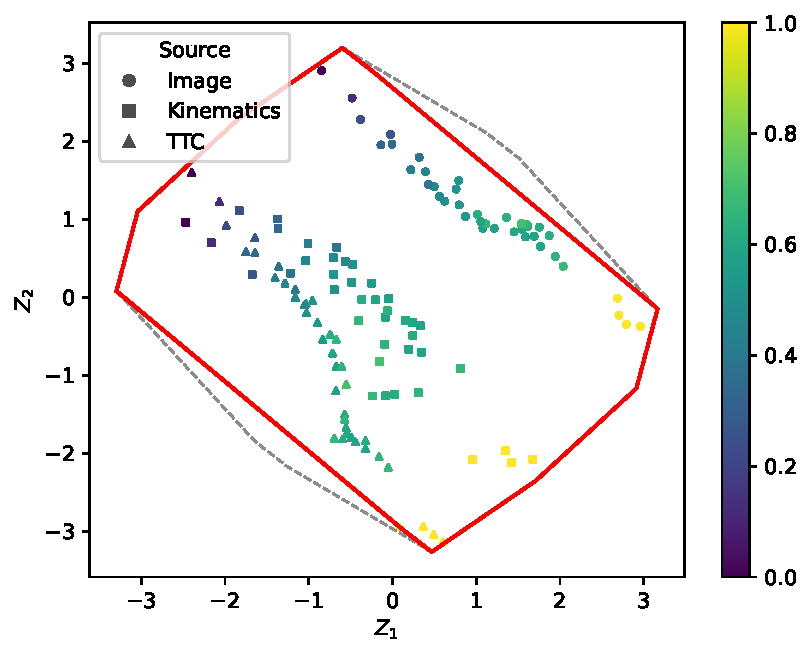
\includegraphics[width=.91\linewidth]{figures/results/single-envs/highway/2_baseline_speed_snr.pdf}
      {\tiny\ttfamily baseline-speed-snr\par}
    \end{minipage} \\
    \begin{minipage}[t]{.29\textwidth}
      \centering
      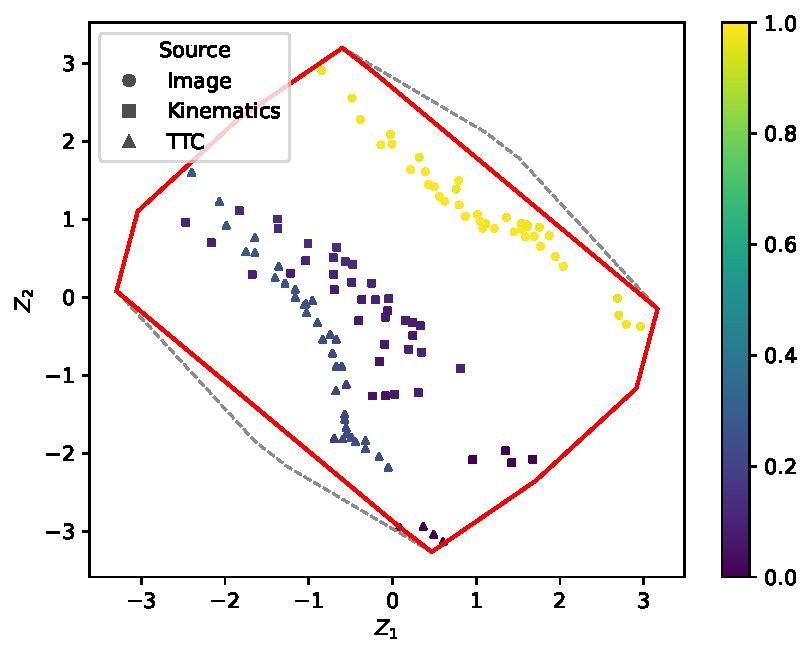
\includegraphics[width=.91\linewidth]{figures/results/single-envs/highway/2_baseline_obs_volatility_mean.pdf}
      {\tiny\ttfamily baseline-obs-volatility-mean\par}
    \end{minipage} &
    \begin{minipage}[t]{.29\textwidth}
      \centering
      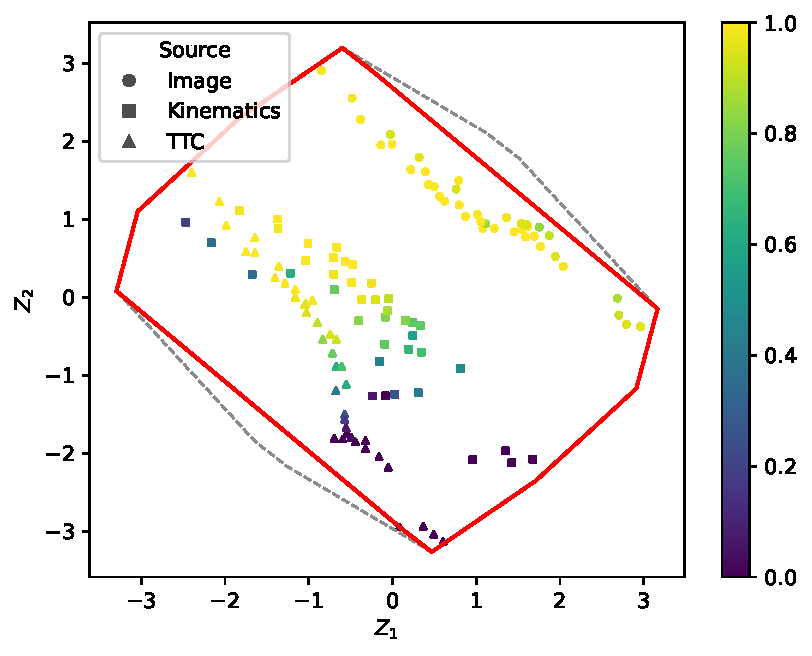
\includegraphics[width=.91\linewidth]{figures/results/single-envs/highway/2_state_entropy.pdf}
      {\tiny\ttfamily state-entropy\par}
    \end{minipage} &
    \begin{minipage}[t]{.29\textwidth}
      \centering
      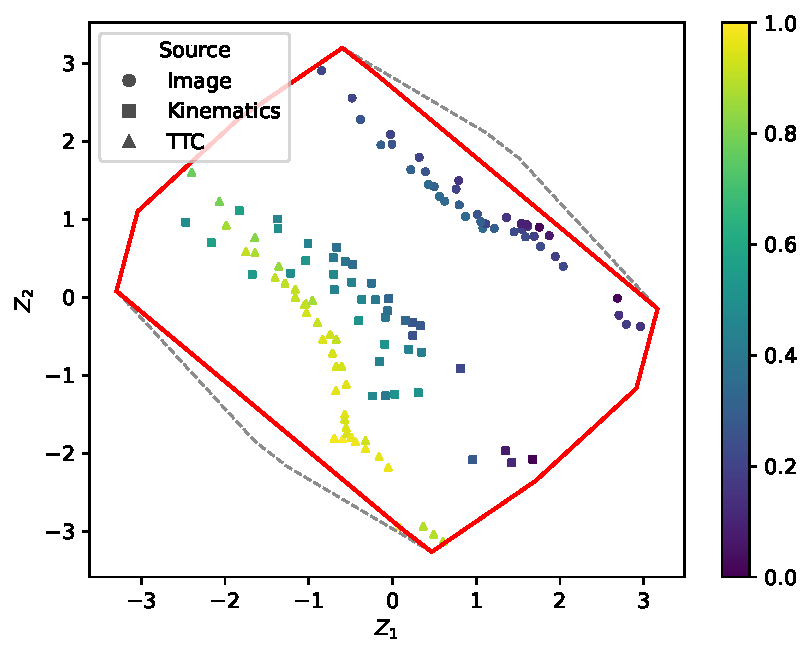
\includegraphics[width=.91\linewidth]{figures/results/single-envs/highway/2_action_state_discontinuity_p95.pdf}
      {\tiny\ttfamily action-state-discontinuity-p95\par}
    \end{minipage}
  \end{tabular}
  \endgroup
\end{frame}

\begin{frame}{Individual Environments}{Highway Selector Algorithm Choices}
  \begin{columns}[c,onlytextwidth]
    \column{.58\textwidth}
      \centering
      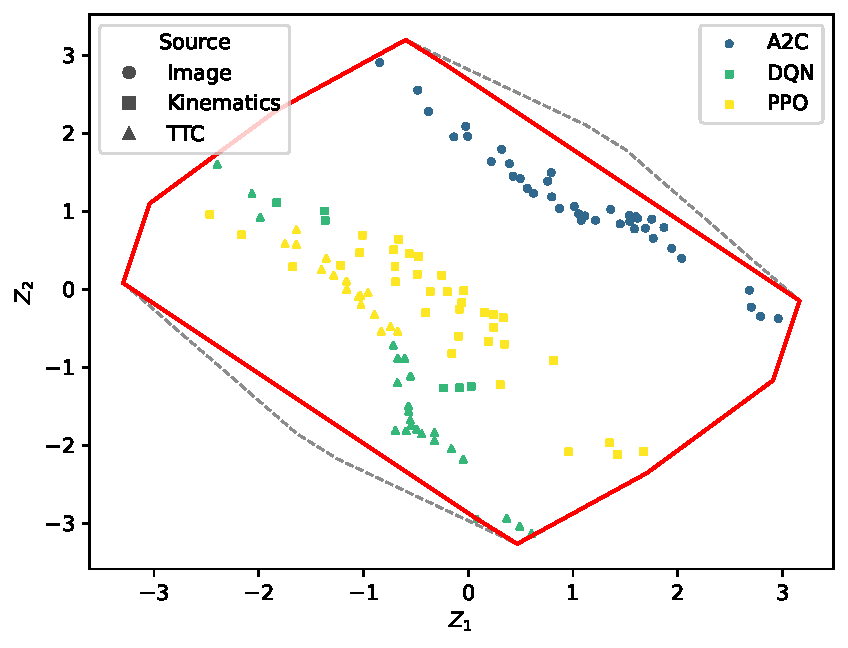
\includegraphics[width=\linewidth]{figures/results/single-envs/highway/6_svm_port.pdf}

    \column{.38\textwidth}
      \scriptsize
      \begin{tabular}{@{}lccc@{}}
        \toprule
        \textbf{Algorithms} & \textbf{Avg.} & \textbf{Std.} & \textbf{Success} \\
        \midrule
        A2C & 0.587 & 0.379 & 0.425 \\
        DQN & 0.512 & 0.488 & 0.467 \\
        PPO & 0.648 & 0.386 & 0.675 \\
        \textbf{Selector} & 0.660 & 0.403 & \textbf{0.750} \\
        Oracle & 0.691 & 0.401 & 1.000 \\
        \bottomrule
      \end{tabular}
  \end{columns}
\end{frame}

\subsection{Multiple Environments}
\begin{frame}{Multiple Environments}{\ttfamily{HighwayEnv} Discrete-Action Environments Projection}
% Sources, best-performing algos
% table of performance
\end{frame}

\subsection{Multiple Environments}
\begin{frame}{Multiple Environments}{All Continuous-Action Environments Projection}
% Sources, best-performing algos
% table of performance
\end{frame}

\subsection{Domain-Specific Characteristics}
\begin{frame}{Domain-Specific Characteristics}{\ttfamily{HighwayEnv} Discrete-Action Environments Projection: %
No domain-specific metafeatures}
  By removing all domain-specific metafeatures, we study their impact on the ability to %
  separate algorithms.

  \vspace{.45em}
  \begin{columns}[c,onlytextwidth]
    \column{.49\textwidth}
      \centering
      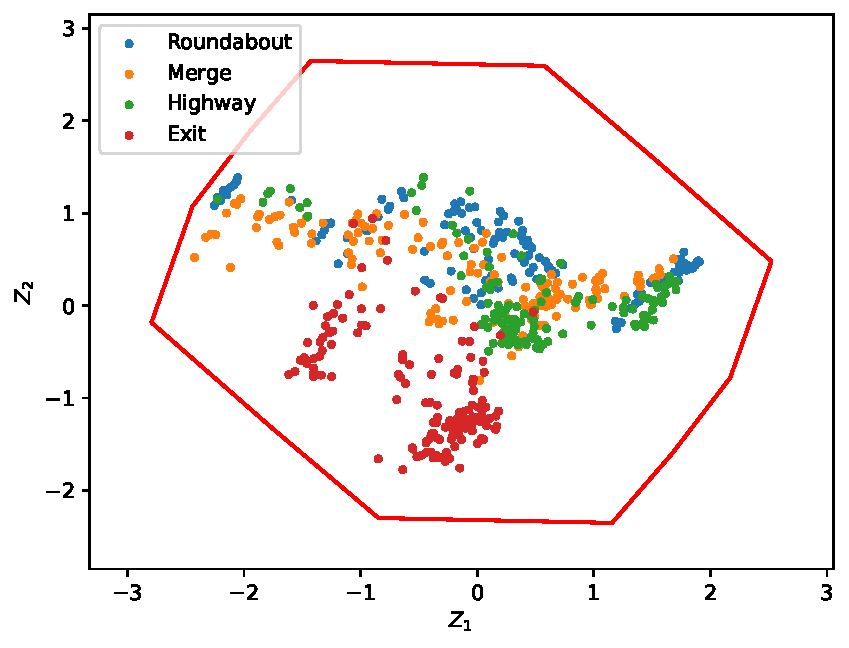
\includegraphics[width=\linewidth]{figures/results/edsm/7_sources.pdf}

    \column{.49\textwidth}
      \centering
      \scriptsize
      \begin{tabular}{@{}lccc@{}}
        \toprule
        \textbf{Algorithms} & \textbf{Avg.} & \textbf{Std.} & \textbf{Success} \\
        \midrule
        A2C & 1.266 & 1.351 & 0.597 \\
        DQN & 1.009 & 1.920 & 0.458 \\
        PPO & 1.419 & 2.065 & 0.648 \\
        \textbf{Selector} & 1.551 / 1.467 & 1.598 / 2.065 & 0.725 / \textbf{0.678} \\
        Oracle & 1.780 & 2.347 & 1.000 \\
        \bottomrule
      \end{tabular}
  \end{columns}
\end{frame}

\section{Conclusions}
% Analyzing individual environments provides context for multi-environment projections.
% Results based on multiple environments provide more generalizable results.
\subsection{Contributions}
\begin{frame}{Contributions}
\end{frame}

\subsection{Future Work}
\begin{frame}{Future Work}
\end{frame}

\section*{Extras}
\begin{frame}{Acknowledgment}
\end{frame}

\begin{frame}[allowframebreaks]{References}
  \printbibliography[heading=none]
\end{frame}

\end{document}
